\documentclass[12pt]{article}
\usepackage[top=1in, bottom=1in, left=1in, right=1in]{geometry}

\usepackage{setspace}
\onehalfspacing

\usepackage{amssymb}
%% The amsthm package provides extended theorem environments
\usepackage{amsthm}
\usepackage{epsfig}
\usepackage{times}
\renewcommand{\ttdefault}{cmtt}
\usepackage{amsmath}
\usepackage{graphicx} % for graphics files
\usepackage{tabu}

% Draw figures yourself
\usepackage{tikz} 

% The float package HAS to load before hyperref
\usepackage{float} % for psuedocode formatting
\usepackage{xspace}

% from Denovo Methods Manual
\usepackage{mathrsfs}
\usepackage[mathcal]{euscript}
\usepackage{color}
\usepackage{array}

\usepackage[pdftex]{hyperref}
\usepackage[parfill]{parskip}

\usepackage{enumerate, paralist, placeins}
%---------------------------------------------------------------------------
%---------------------------------------------------------------------------
\begin{document}
\begin{center}
{\bf NE 155/255, Fall 2019 \\
Parallel Computing Overview \\
December 6, 2019 
}
\end{center}

Lecture notes adapted from Blaise Barney's ``Introduction to Parallel
Computing'' tutorial at
\url{https://computing.llnl.gov/tutorials/parallel_comp/} .

\subsection*{Serial Computing}

Traditionally, we tend to think about algorithms in a serial way, and it has
followed that software has been historically written serially:

\begin{compactitem}
\item Problem broken into discrete series of instructions
\item Instructions executed sequentially, one after another
\item Single processor used for execution
\item Only one instruction may execute at any point in time
\end{compactitem}

\begin{figure}[hbt!]
\centering
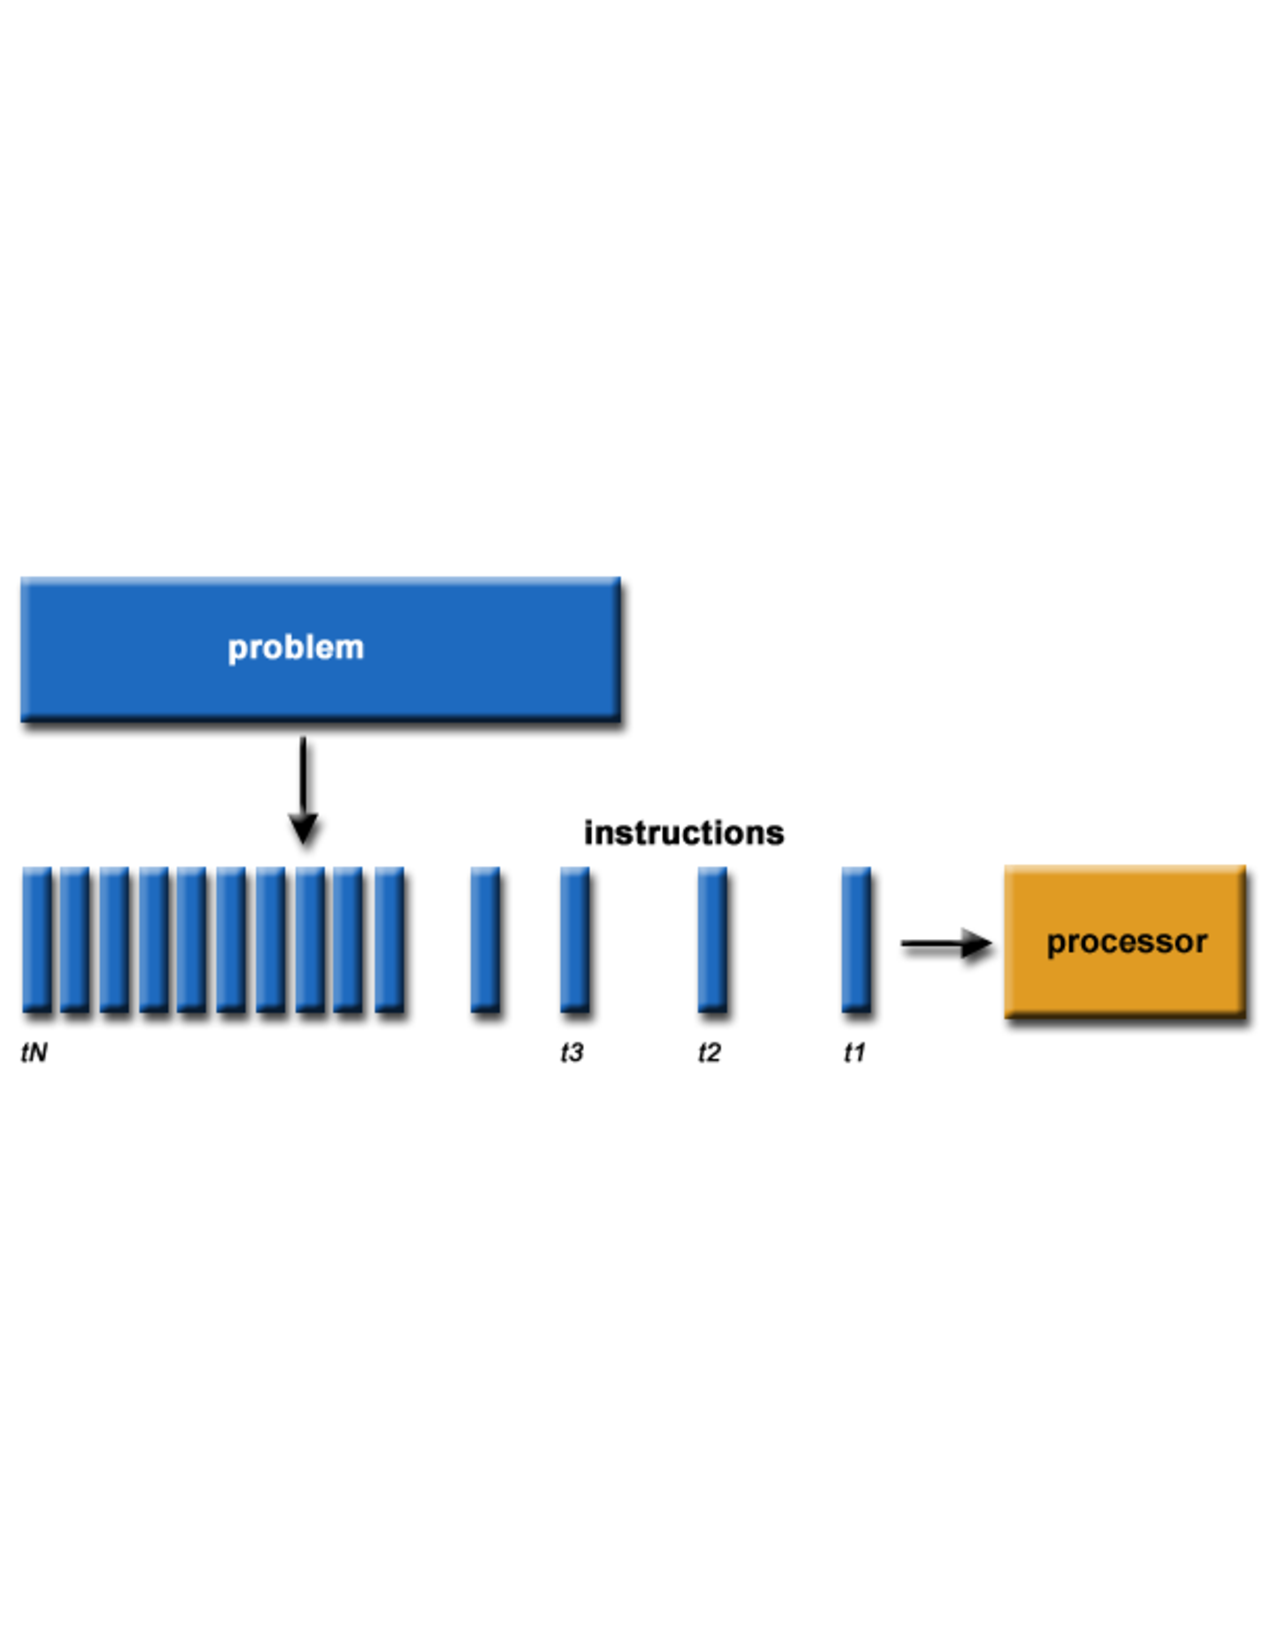
\includegraphics[width=0.5\textwidth]{serial-problem.pdf}
\caption{Serial computing.}
\end{figure}

\FloatBarrier
\subsection*{Parallel Computing}

On the other hand, parallel computing is the simultaneous use of multiple
compute resources to solve a computational problem:

\begin{compactitem}
\item Problem broken into discrete parts that can be solved concurrently
\item Each part further broken down into series of instructions
\item Instructions from each part execute simultaneously on different
      processors
\item Some overall control/coordination mechanism is used to collect results
\end{compactitem}

In order to use parallel computing techniques, we impose requirements on the
computational problem that we're trying to solve.. The problem should be able to:

\begin{compactitem}
\item Break down into discrete work pieces that can be solved simultaneously;
\item Execute multiple program instructions at any point in time;
\item Be solved in less time with multiple compute resources than with a single
      compute resource.
\end{compactitem}

\begin{figure}[!htb]
\centering
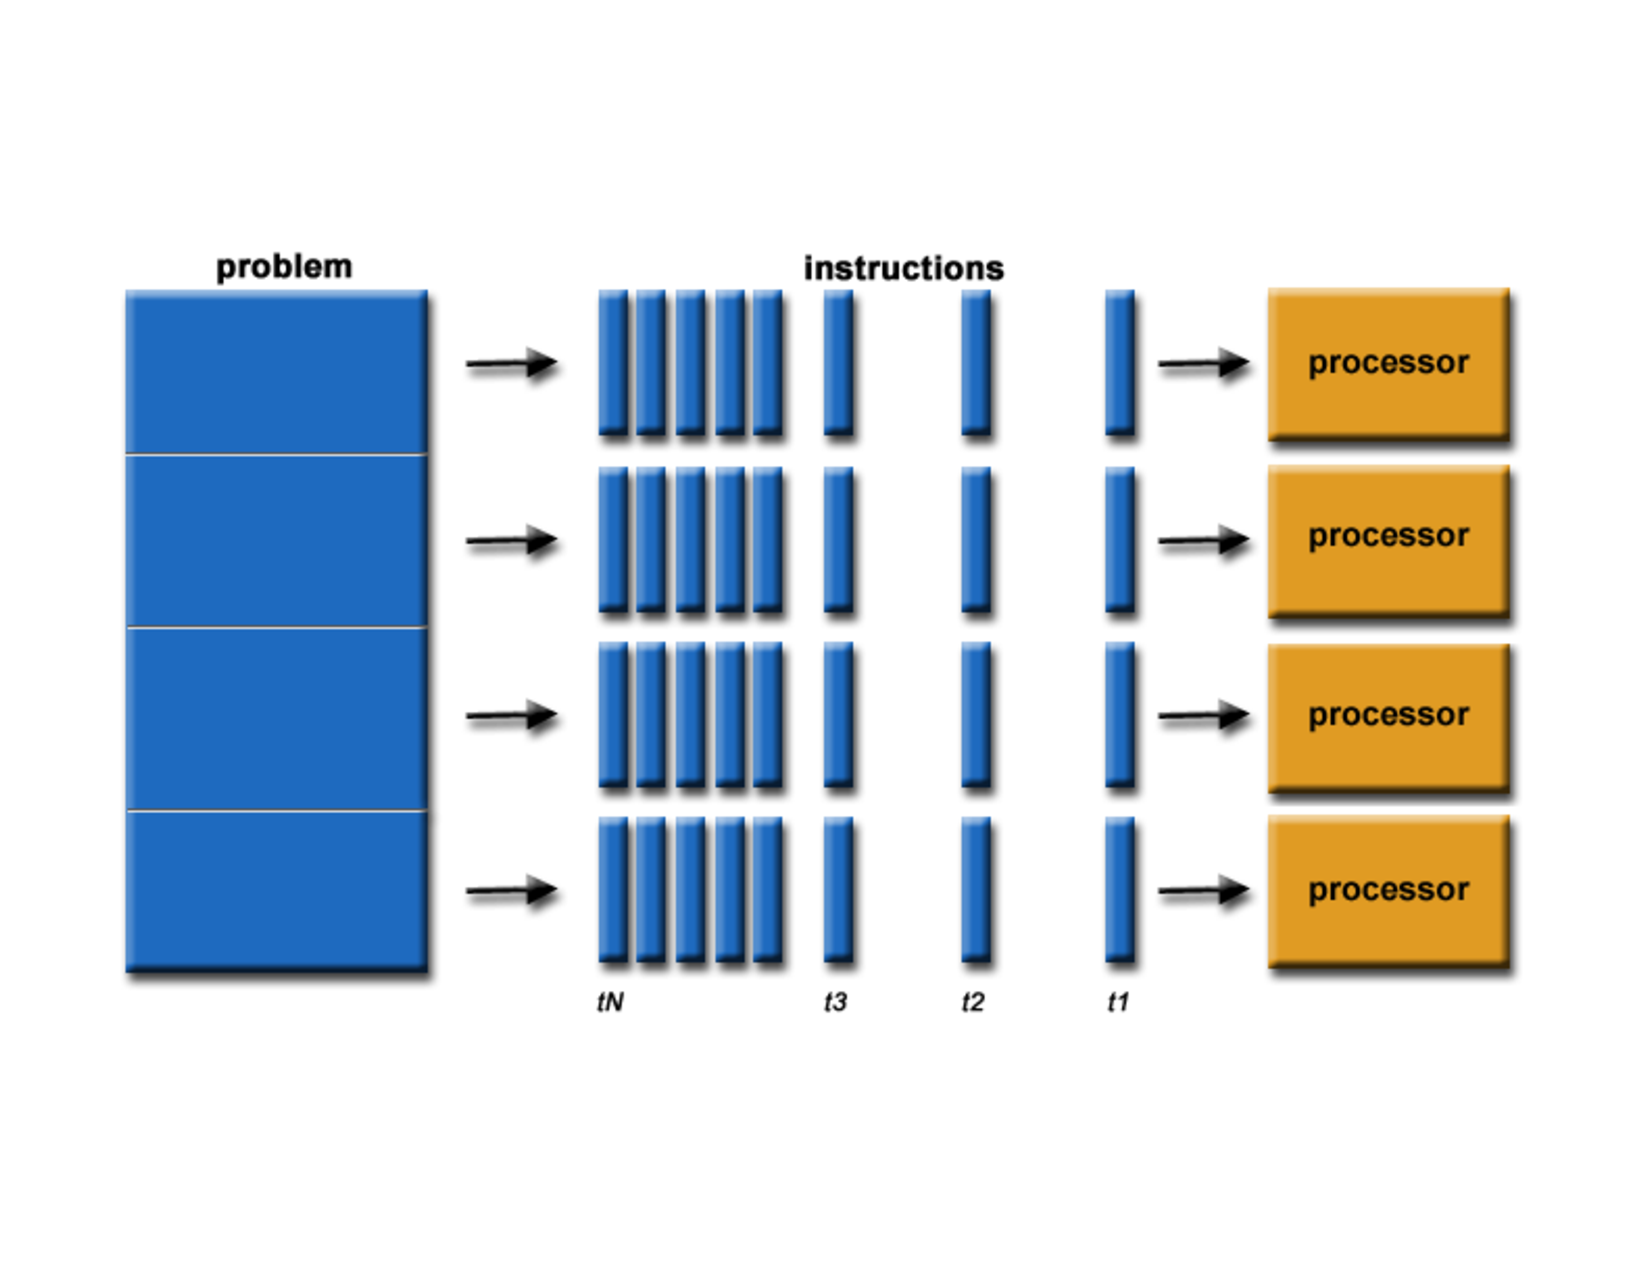
\includegraphics[width=0.5\textwidth]{parallel-problem.pdf}
\caption{Parallel computing.}
\end{figure}

\FloatBarrier
\subsection*{Parallel Computers}

Parallel compute resources can be a single computer with multiple processors or
a number of computers connected by a network. Today, any given standalone
computer is typically parallel from a hardware perspective; it has multiple
functional units, multiple execution units (processors), and mulitple hardware
threads.

Networks connect multiple standalone computers (``nodes'') to make larger
parallel computer ``clusters''. So, each compute node is a multiprocessor
parallel computer by itself, and then multiple compute nodes are networked
together for even more parallelism.

\subsubsection*{Flynn's Taxonomy}

There are different ways to classify parallel computers; one of the more
widely-used classifications is called Flynn's Taxonomy. Flynn's Taxonomy defines
the two independent dimensions of ``instruction stream'' and ``data stream``
and holds that aech dimension can have only one of two possible states
``single'' or ``multiple''. This gives us 4 possible classifications:

\begin{compactitem}
\item \textbf{SISD}: single instruction, single data
\item \textbf{SIMD}: single instruction, multiple data
\item \textbf{MISD}: multiple instruction, single data
\item \textbf{MIMD}: multiple instruction, multiple data
\end{compactitem}

\begin{figure}[!htb]
\centering
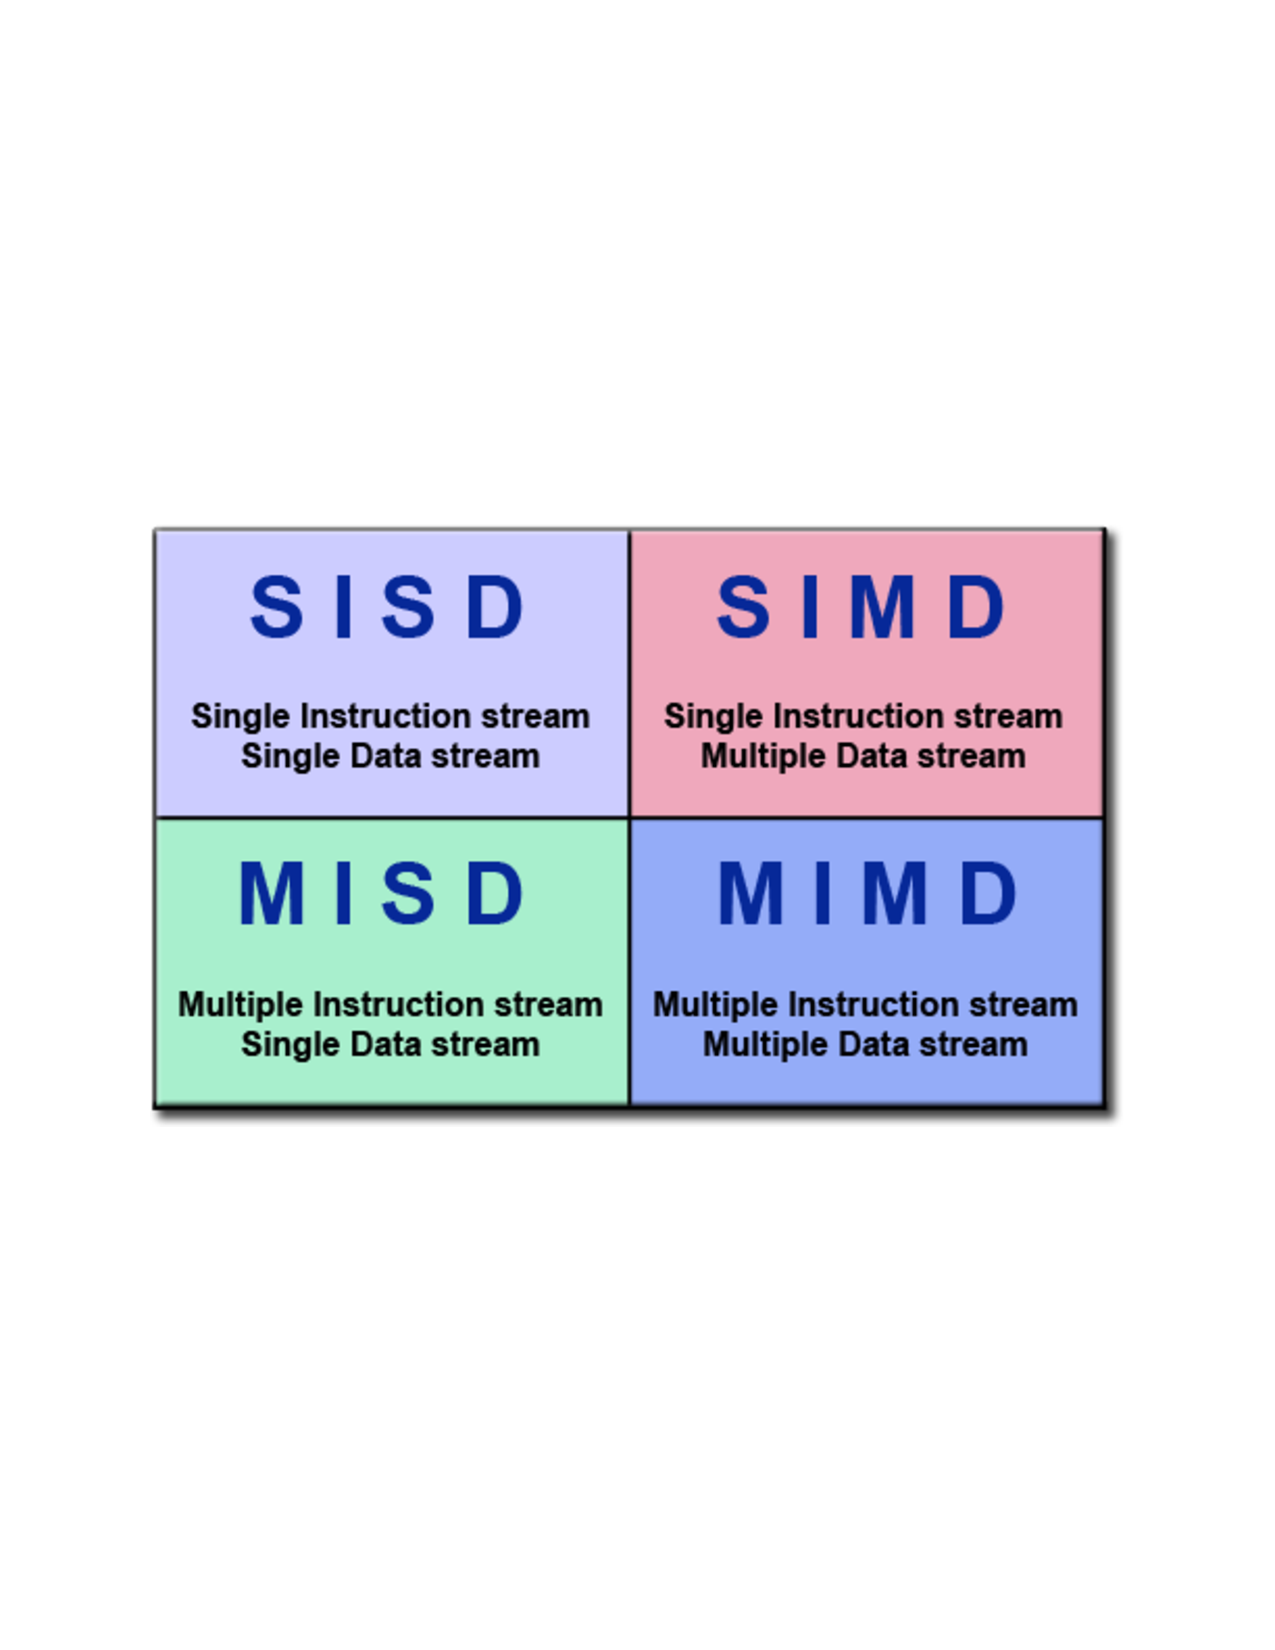
\includegraphics[width=0.5\textwidth]{flynns.pdf}
\end{figure}

\pagebreak
\paragraph*{SISD}

\begin{compactitem}
\item Serial computer
\item Only one instruction stream acted on by the CPU during any one clock
      cycle
\item Only one data stream used as input during any one clock cycle
\item Deterministic execution
\end{compactitem}

\paragraph*{SIMD}

\begin{compactitem}
\item Parallel computer
\item All processing units execute the same instruction at a given clock cycle
\item Each processing unit can operate on a different data unit
\item Synchronous (lockstep) and deterministic execution
\item Best suited for problems with a high degree of regularity (e.g., image
      processing)
\item Most modern computers use SIMD instructions and execution units
\end{compactitem}

\paragraph*{MISD}

\begin{compactitem}
\item Parallel computer
\item Each processor operates on data independently via separate instruction
      streams
\item A single data stream is fed into multiple processors
\item Few actual examples of this have ever existed
\end{compactitem}

\paragraph*{MIMD}

\begin{compactitem}
\item Parallel computer
\item Every processor may be executing a different instruction stream
\item Every processor may be working with a different data stream
\item Execution can be synchronous or asynchronous, deterministic or
      non-deterministic
\item Many MIMD architectures include SIMD execution sub-components
\item Most current supercomputers fall into this category
\end{compactitem}

\pagebreak
\subsection*{Parallel Programming Models}

\subsubsection*{Shared Memory (without Threads)}

\begin{compactitem}
\item Tasks share a common address space, which they read and write to
      asynchronously
\item Mechanisms like as locks are used to control access to the shared memory,
      resolve contentions, and to prevent race conditions and deadlocks
\item No need to specify explicitly the communication of data between tasks
\item All processes see and have equal access to shared memory
\item In terms of performance, it becomes more difficult to understand and 
      manage data locality
\end{compactitem}

\subsubsection*{Threading}

\begin{compactitem}
\item Threading is a type of shared memory programming
\item A single ``heavy weight'' process can have multiple ``light weight''
      concurrent execution paths
\item Threads communicate with each other through global memory (updating
      address locations)
\item Synchronization constructs are needed to ensure that more than one thread
      is not updating the same global address at any time
\item Commonly-used implementations of threads are \textbf{POSIX threads} and 
      \textbf{OpenMP}
\end{compactitem}

\subsubsection*{Distributed Memory}

\begin{compactitem}
\item Also called the ``message-passing'' model
\item This model uses a set of tasks that use their own local memory during
      computation
\item Multiple tasks can reside on the same standalone computer and/or across a
      network of computers
\item Tasks exchange data through communications by sending and receiving
      messages
\item Data transfer usually requires cooperative operations to be performed by
      each process (e.g., a ``send'' operation must have a matching ``receive''
      operation)
\item \textbf{Message Passing Interface (MPI)} is the de facto standard for
      distributed computing
\end{compactitem}

\pagebreak
\subsection*{Designing Parallel Programs}

\textbf{Understand the problem and the program.} The first step in developing
parallel software is to understand the problem that your wish to solve in
parallel. If you're starting with serial code, you must also understand the
existing code. Before spending any time attempting to develop a parallel
solution for a problem, determine whether or not the problem is one that can
actually be parallelized.

\begin{itemize}
\item Partitioning
      \begin{itemize}
      \item Break the problem into discrete ``chunks'' of work that can be
            distributed to multiple tasks
      \item Domain decomposition and functional decomposition
      \end{itemize}
\item Communications
      \begin{itemize}
      \item The need for communications between tasks depends upon your problem
      \item ``Embarrassingly parallel'' problems need little to no
            communication
      \item Communication always incurs some overhead
      \item Latency versus bandwidth
      \item Synchronous (blocking) versus asynchronous (non-blocking)
      \end{itemize}
\item Synchronization
      \begin{itemize}
      \item Managing the sequence of work and the tasks performing it is a
            critical design consideration
      \item Can be a significant factor in program performance
      \item Often requires ``serialization'' of segments of the program
      \item Barrier, lock/semaphore, synchronous communications
      \end{itemize}
\item Data dependencies
      \begin{itemize}
      \item A dependence exists between program statements when the order of
            statement execution affects the results of the program
      \item A data dependence results from multiple use of the same location(s)
            in storage by different tasks
      \item Dependencies are one of the primary inhibitors to parallelism
      \end{itemize}
\item Load balancing
      \begin{itemize}
      \item Distributing approximately equal amounts of work among tasks so
            that all tasks are kept busy all of the time
      \item Minimization of task idle time
      \item Important for performance reasons; the slowest task will determine
            overall performance
      \end{itemize}
\item Granularity
      \begin{itemize}
      \item Qualitative measure of the ratio of computation to communication
      \item Fine-grained versus coarse-grained parallelism
      \item Most efficient granularity is dependent on the algorithm and the
            hardware environment in which it runs
      \end{itemize}
\item I/O
      \begin{itemize}
      \item Generally regarded as inhibitor to parallelism
      \item I/O operations require orders of magnitude more time than memory
            operations
      \end{itemize}
\item Debugging
      \begin{itemize}
      \item Can be incredibly difficult, especially as codes scale
      \end{itemize}
\item Performance Analysis and Tuning
      \begin{itemize}
      \item Much more challenging for parallel software than serial code
      \end{itemize}
\end{itemize}

\end{document}
